
\documentclass[submit]{harvardml}


\course{CS181-S19}
\assignment{Assignment \#4}
\duedate{11:59pm April 5, 2019}

\usepackage[OT1]{fontenc}
\usepackage[colorlinks,citecolor=blue,urlcolor=blue]{hyperref}
\usepackage[pdftex]{graphicx}
\usepackage{subfig}
\usepackage{fullpage}
\usepackage{amsmath}
\usepackage{amssymb}
\usepackage{color}
\usepackage{todonotes}
\usepackage{listings}
\usepackage{common}
\usepackage{bm}

\usepackage[mmddyyyy,hhmmss]{datetime}

\definecolor{verbgray}{gray}{0.9}

\lstnewenvironment{csv}{%
  \lstset{backgroundcolor=\color{verbgray},
  frame=single,
  framerule=0pt,
  basicstyle=\ttfamily,
  columns=fullflexible}}{}

\begin{document}
\begin{center}
{\Large Homework 4: Clustering and EM}\\
\end{center}


This homework assignment focuses on different unsupervised learning
methods from a theoretical and practical standpoint.  In Problem 1,
you will explore Hierarchical Clustering and experiment with how the
choice of distance metrics can alter the behavior of the algorithm. In
Problem 2, you will derive from scratch the full
expectation-maximization algorithm for fitting a Poisson mixture
model. In Problem 3, you will implement PCA on a dataset of
handwritten images and analyze the latent structure learned by this
algorithm.

There is a mathematical component and a programming component to this
homework.  Please submit your PDF, tex, and Python files to Canvas,
and push all of your work to your GitHub repository. If a question
requires you to make any plots, please include those in the writeup.

\newpage

\begin{problem}[Hierarchical Clustering, 7 pts]
  
At each step of hierarchical clustering, the two most similar clusters
are merged together. This step is repeated until there is one single
group. We saw in class that hierarchical clustering will return a
different result based on the pointwise-distance and cluster-distance
that is is used. In this problem you will examine different choices of
pointwise distance (specified through choice of norm) and cluster
distance, and explore how these choices change how the HAC algorithm
runs on a toy data set.

  
 Consider the following four data points in $\reals^2$, belonging to three clusters: the
  black cluster consisting of $\boldx_1 = (0.1, 0.5) $ and $\boldx_2 = (0.35, 0.75))$,
  the red cluster consisting of $\boldx_3 = (0.28, 1.35)$, and the blue cluster
  consisting of $\boldx_4 = (0, 1.01)$.

  \begin{center} \includegraphics[scale=.3]{scatterplot.png} \end{center}


  Different pointwise distances $d(\boldx, \boldx') = \|\boldx - \boldx'\|_p$
  can be used.  Recall the definition of the
  $\ell_1$, $\ell_2$, and $\ell_{\infty}$ norm:
  \begin{eqnarray*}
     \| \mathbf{x} \|_1 = \sum_{j = 1}^m |x_i| \quad \quad\quad \| \mathbf{x} \|_2 = \sqrt{\sum_{j = 1}^m x_i^2 } \quad\quad\quad
     \| \mathbf{x} \|_{\infty} = \max_{j \in \{1, \ldots, m\}} |x_j|\\
  \end{eqnarray*}
  
  Also recall the definition of min-distance, max-distance,
  centroid-distance, and average-distance between two clusters (where $\bmu_{G}$
is the center of a cluster $G$):
%
\begin{eqnarray*}
    d_{\text{min}}(G, G') &=& \min_{\boldx  \in G, \boldx' \in G'} d(\boldx, \boldx')\\
    d_{\text{max}}(G, G') &=& \max_{\boldx  \in G, \boldx' \in G'} d(\boldx, \boldx')\\
    d_{\text{centroid}}(G, G') &=&  d(\bmu_{G}, \bmu_{G'})\\
    d_{\text{avg}}(G, G') &=&\frac{1}{|G| |G'|} \sum_{\boldx \in G}\sum_{\boldx'  \in G'} d(\boldx, \boldx')\\
  \end{eqnarray*}

  \begin{enumerate}
  \item Draw the 2D unit sphere for each norm,
  defined as $\mathcal{S} = \{\boldx \in \mathbb{R}^2: \|\boldx\| = 1 \}$. Feel free to do
  it by hand, take a picture and include it in your pdf.
\item  For each norm ($\ell_1, \ell_2, \ell_\infty$) and each clustering distance, specify which two clusters would
  be the first to merge.
\item Draw the complete dendrograms showing the order of agglomerations for the $\ell_2$ norm and each of the clustering distances. We have provided some code to make this easier for you. You are not required to use it.
  \end{enumerate}


\end{problem}

\subsection*{Solution}

\begin{enumerate}
\item The unit spheres are drawn below. They are a diamond, circle, and square for $l_1$, $l_2$, and $l_\infty$ respectively.

\begin{center}
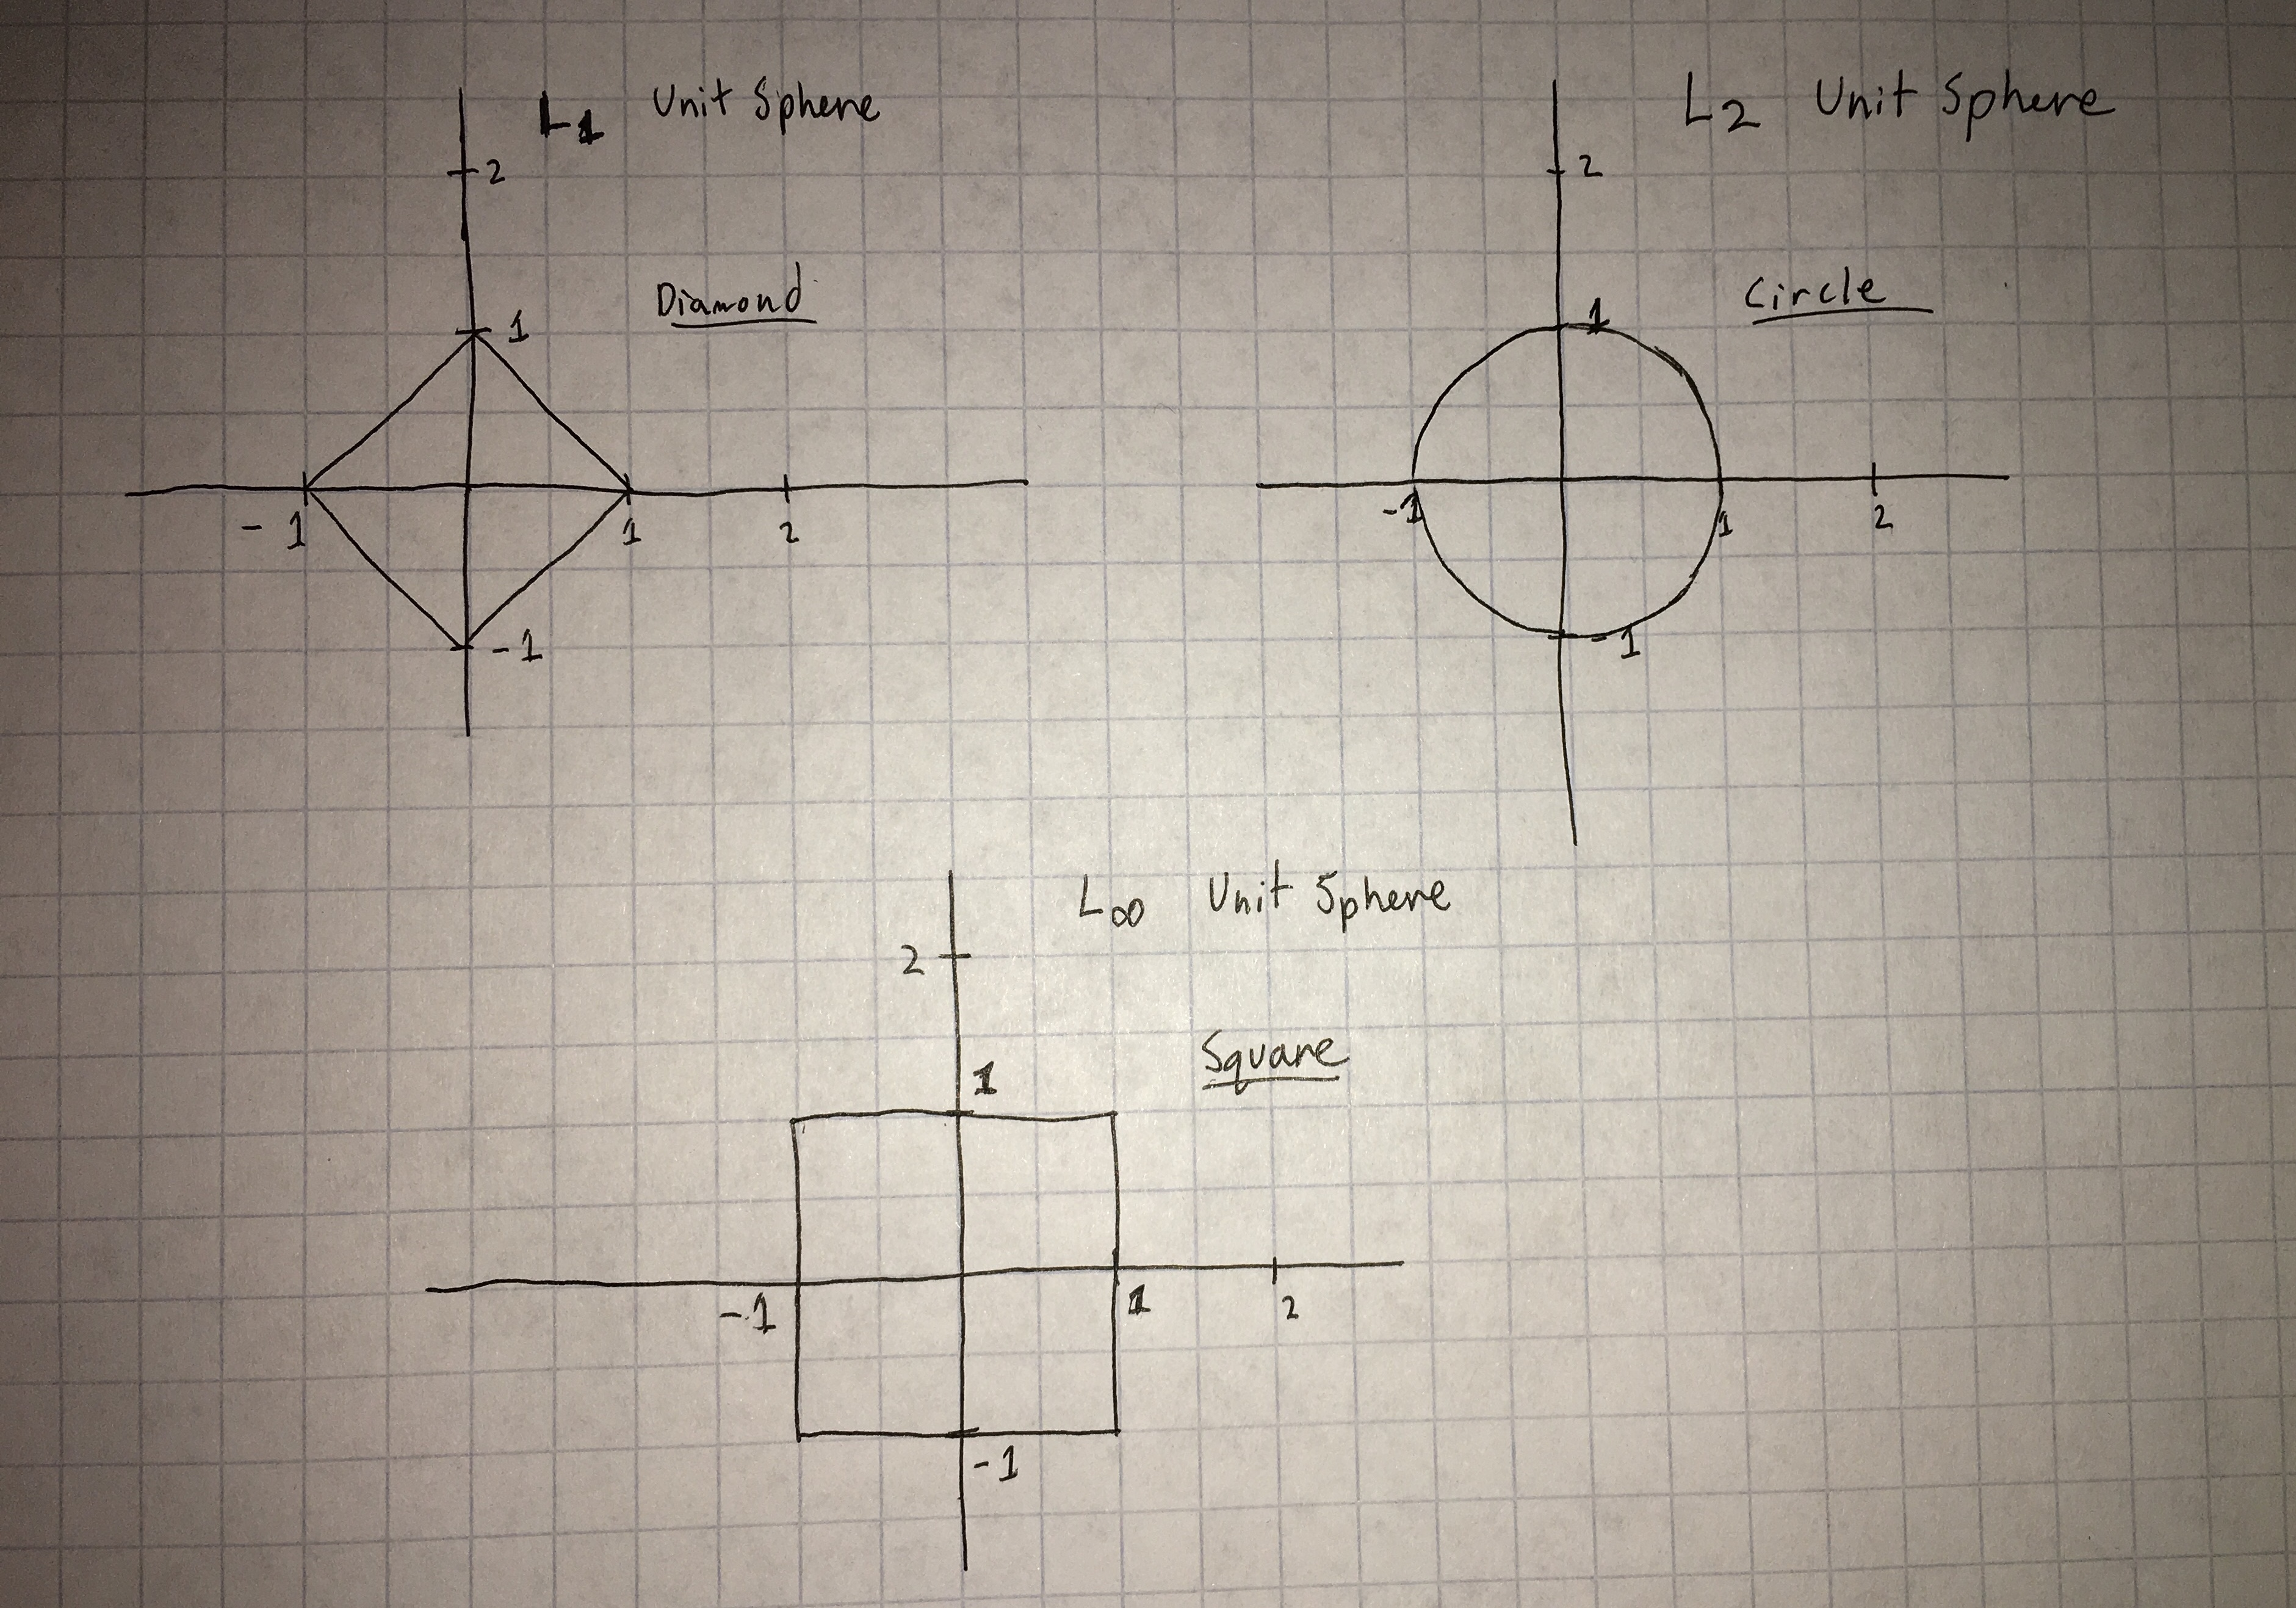
\includegraphics[scale=0.1]{spheres}
\end{center}
\item See the table below for my sesults of which two clusters would merge first under each combination of distance metric and cluster center.

\begin{tabular}{ |p{3cm}||p{3cm}|p{3cm}|p{3cm}|  }
 \hline
 \multicolumn{4}{|c|}{Part 2: First Two Clusters to Merge} \\
 \hline
 & $l_1$ distance & $l_2$ distance & $l_{\infty}$ distance\\
 \hline
 Min & Black and Blue    & Black and Blue &   Red and Blue \\
 Max &   Black and Blue  & Red and Blue   & Red and Blue \\
 Centroid & Black and Blue & Red and Blue &   Red and Blue \\
 Average   & Black and Blue & Red and Blue &  Red and Blue \\
 \hline
\end{tabular}

\item Below are the dendrograms, which I attempted to draw to scale. The distance which is hard to read in the ``L2, Centroid Dist'' dendrogram is 0.561.

\begin{center}
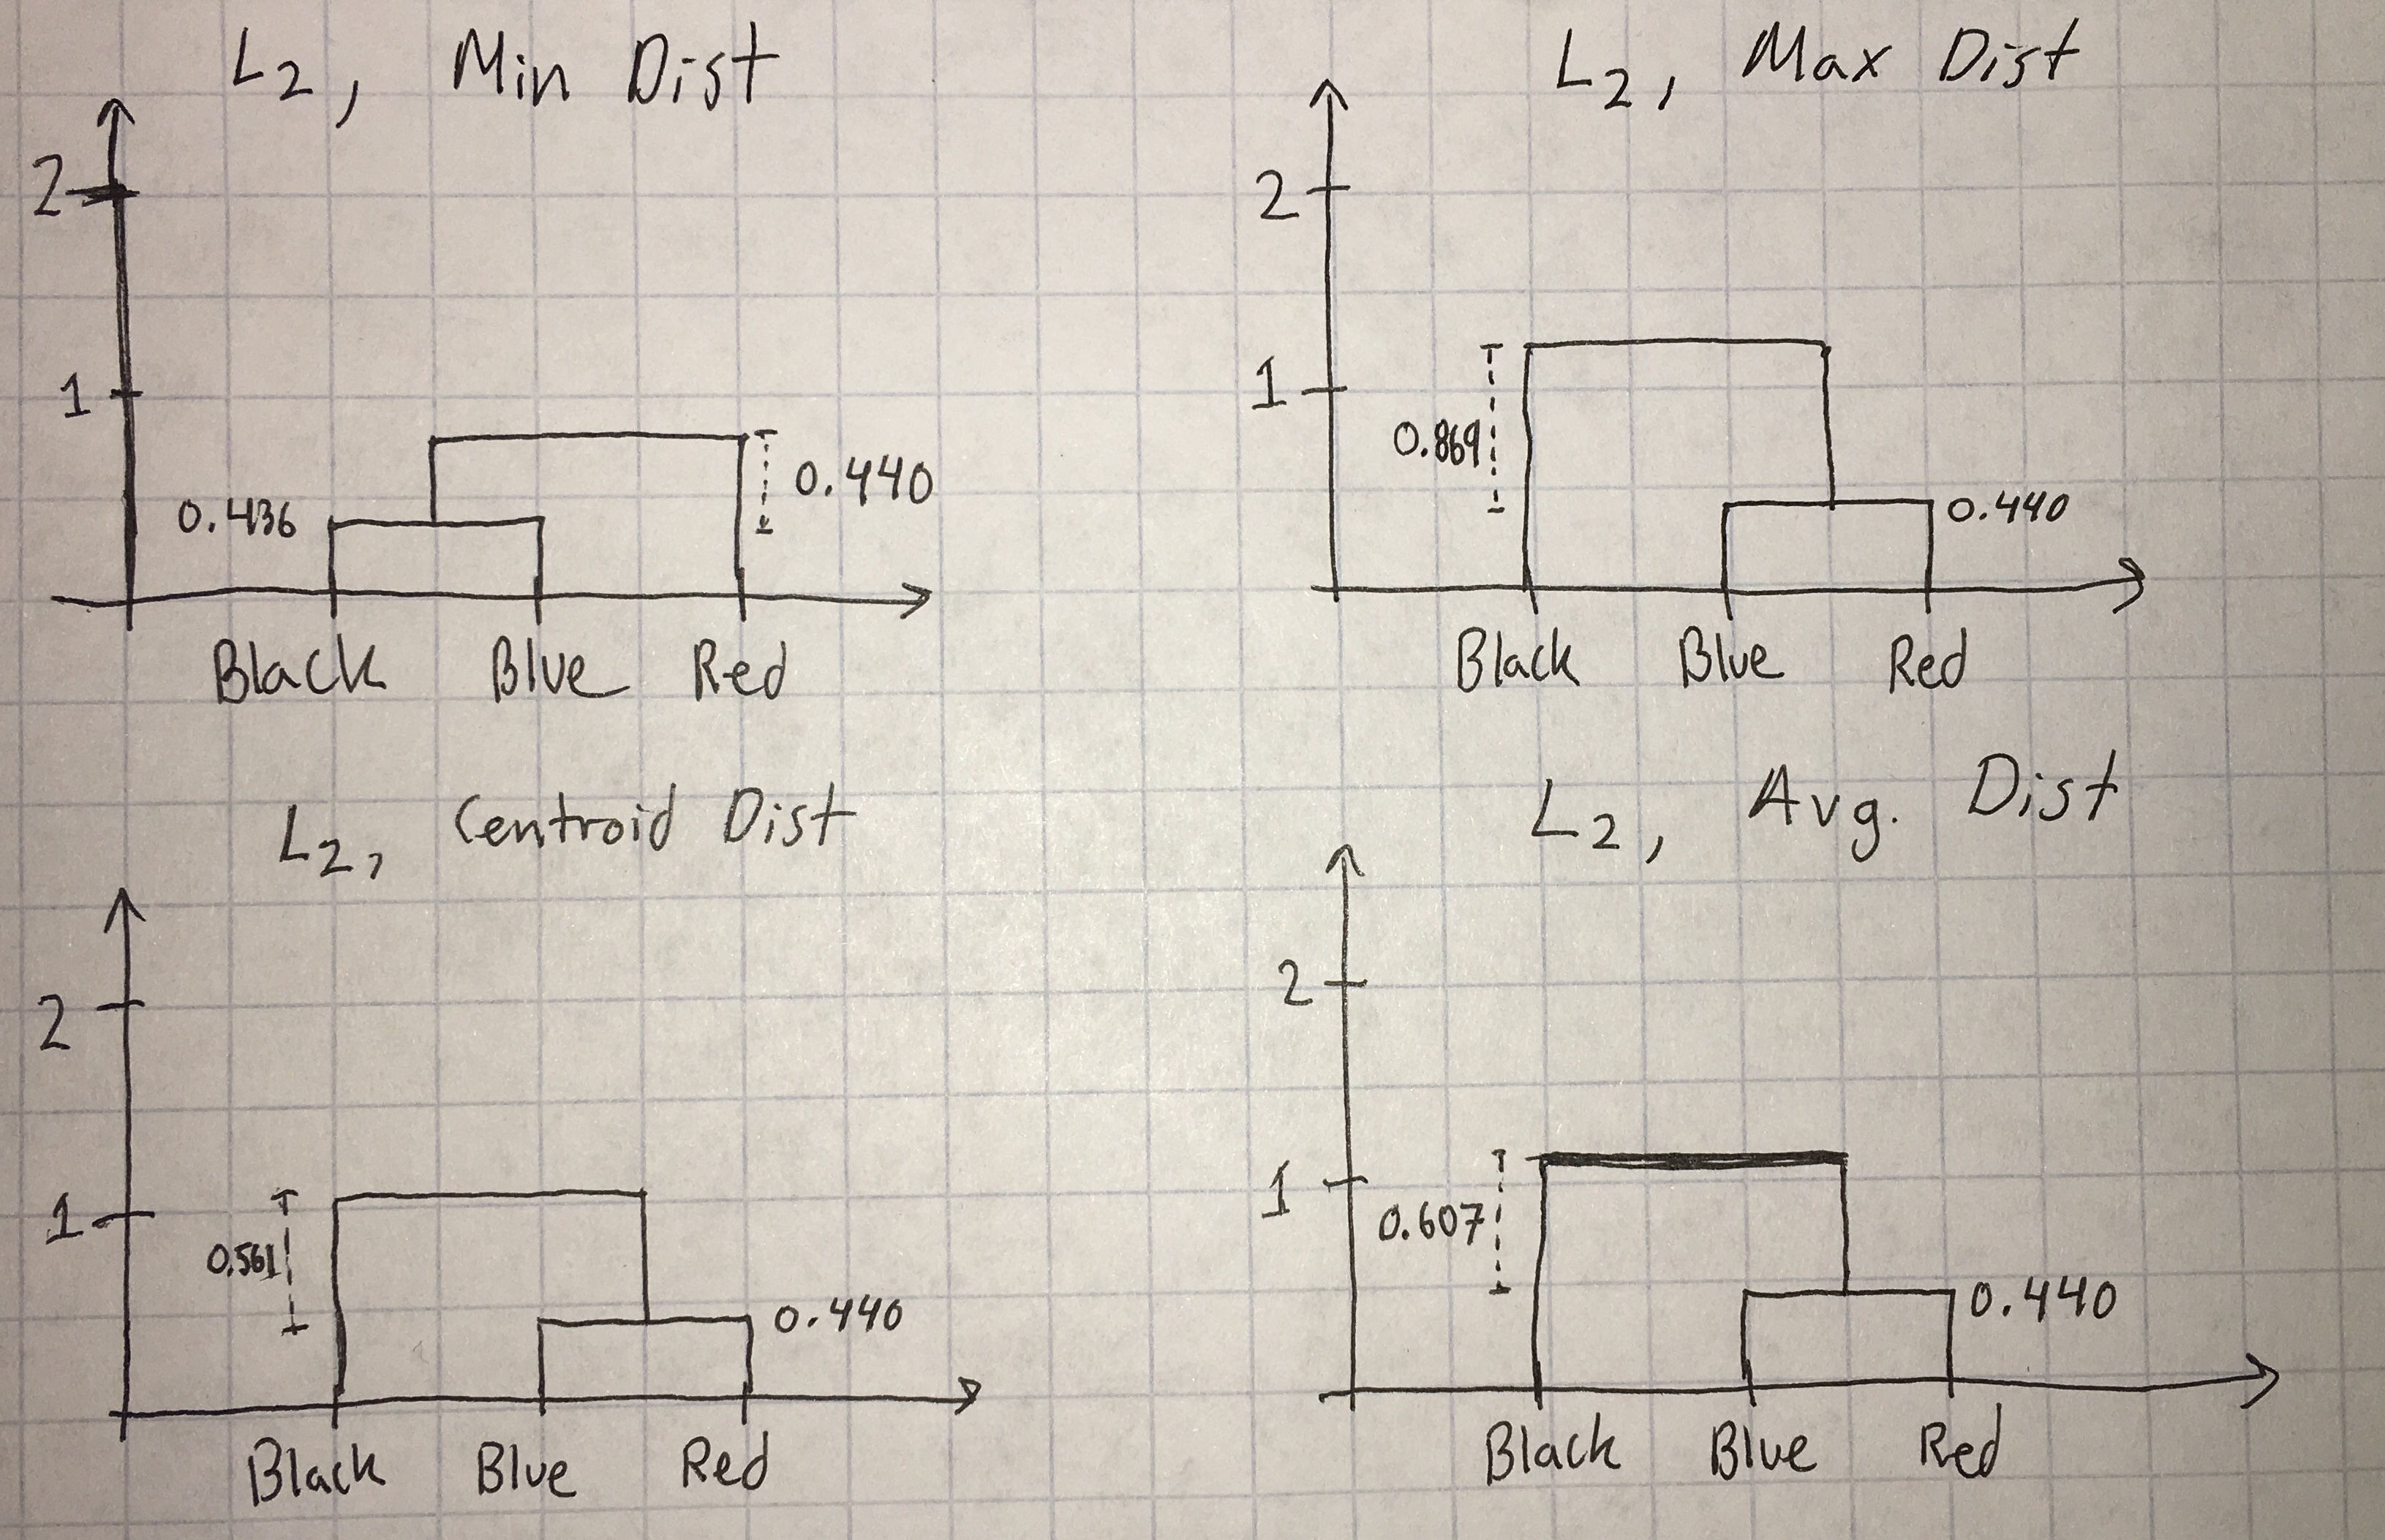
\includegraphics[scale=0.15]{den}
\end{center}

\end{enumerate}

\newpage 

\begin{problem}[Expectation-Maximization for Poisson Mixture Models, 7pts]

In this problem we will explore expectation-maximization for the
Poisson Mixture model.  Each observation $\boldx_n$ is a vector in the
non-negative integers $\mathbb{Z}^{*}$.  We posit that each
observation comes from \emph{one} mixture component.  For this
problem, we will assume there are $K$~components. Each component $k
\in \{1, \ldots, K\}$ will be associated with a mean vector $\lambda_k
\in R^{+}$.  Finally let the (unknown) overall mixing proportion of
the components be~$\btheta \in [0,1]^K$, where~${\sum_{k=1}^K
  \btheta_k=1}$.

Our generative model is that each of the~$N$ observations comes from a
single component.  We encode observation $n$'s component-assignment as
a one-hot vector~${\boldz_n \in \{0,1\}^K}$ over components. This
one-hot vector is drawn from~$\btheta$; then, $\boldx_n$ is drawn
from~$\text{Poisson}(\lambda_{z_n} )$, which simply means that if $\boldz_{nj} = 1$ for some $j \in \{1,\ldots, K\}$ (i.e. the $j$th element of $\boldz_n$ equals $1$), then $\boldx_n \sim \text{Poisson}(\lambda_j)$. 

Formally, documents are generated in two
steps:
\begin{eqnarray*}
 \boldz_n &\sim& \text{Categorical}(\btheta) \\
 \boldx_n &\sim& \text{Poisson}(\lambda_{z_n} )
\end{eqnarray*}

  \begin{enumerate}

  \item \textbf{Intractability of the Data Likelihood} We are
    generally interested in finding a set of parameters $\lambda_k$
    that maximize the data likelihood $\log p(\{\boldx_n\}^N_{n=1}|\{\lambda_k\}^K_{k = 1})$.
    Expand the data likelihood to include the necessary sums over
    observations $\boldx_n$ and latents $\boldz_n$.  Why is optimizing this loss
    directly intractable?
    
\item \textbf{Complete-Data Log Likelihood} Define the complete data for this problem to be $D = \{(\boldx_n, \boldz_n)\}_{n=1}^N$. Write out the complete-data negative log likelihood. Note that optimizing this loss is now computationally tractable if we know $\boldz_n$.

\[\mcL(\btheta, \{\lambda_k\}^K_{k=1}) =  -\log p(D \given\btheta, \{\lambda_k\}^K_{k=1}).\] 
    

\item \textbf{Expectation Step}
Our next step is to introduce a mathematical expression for $\boldq_n$, the posterior over the hidden topic variables~$\boldz_n$ conditioned on the observed data $\boldx_n$ with fixed parameters, i.e $p(\boldz_n | \boldx_n; \btheta, \{ \lambda_k \}^K_{k=1})$.

\begin{itemize}
\item  \textbf{Part 3.A } Write down and simplify the expression for $\boldq_n$. 
\item  \textbf{Part 3.B } Give an algorithm for calculating $\boldq_n$ for all $n$, given the observed data~$\{\boldx_n\}^N_{n=1}$ and settings of the parameters~$\btheta$ and~$\{ \lambda_k,  \}^K_{k=1}$.

\end{itemize}

\item \textbf{Maximization Step}
Using the~$\boldq_n$ estimates from the Expectation Step, derive an update for maximizing the expected complete data log likelihood in terms of~$\btheta$ and~$\{ \lambda_k \}^K_{k=1}$.

\begin{itemize}
    \item \textbf{Part 4.A } Derive an expression for the expected complete-data log likelihood in terms of $\boldq_n$.
    \item \textbf{Part 4.B } Find an expression for $\btheta$ that maximizes this expected complete-data log likelihood. You may find it helpful to use Lagrange multipliers in order to enforce the constraint $\sum \theta_k = 1$. Why does this optimized $\btheta$ make intuitive sense?
    \item \textbf{Part 4.C } Apply a similar argument to find the values of $\{\lambda_k
      \}^K_{k = 1}$ that maximizes the expected complete-data log likelihood.
\end{itemize}

\item Suppose that this had been a classification problem, that is,
  you were provided the ``true'' categories $\boldz_n$ of each
  document, and you were going to perform the classification by
  inverting the provided generative model.  Could you reuse any of
  your inference derivations above?  
  
\end{enumerate}


  
\end{problem}

\subsection*{Solution}

\begin{enumerate}

\item Using the law of total probability, we have that for a single data point, $x_n$, the following holds

$$p(x_n|\{\lambda_k\}^K_{k = 1}) =\sum_{j=1}^K p(x_n| z_n = j,\{\lambda_k\}^K_{k = 1}) p(z_n = j)$$

Then, since $x_n|z_n$ is distributed $\textrm{Pois}(\lambda_{z_n})$ and $p(z_n = j) = \bold\theta_j$, we have that

$$p(x_n|\{\lambda_k\}^K_{k = 1}) =\sum_{j=1}^K \frac{\lambda_j^{x_n}e^{-\lambda_j}}{x_n!} \bold\theta_j$$

and thus we have that for all $n$ data points,

$$ p(\{\boldx_n\}^N_{n=1}|\{\lambda_k\}^K_{k = 1}) = \prod_{i=1}^N \sum_{j=1}^K \frac{\lambda_j^{x_i}e^{-\lambda_j}}{x_i!} \bold\theta_j $$

meaning

$$ \boxed{ \log p(\{\boldx_n\}^N_{n=1}|\{\lambda_k\}^K_{k = 1}) = \sum_{i=1}^N \log(\sum_{j=1}^K \frac{\lambda_j^{x_i}e^{-\lambda_j}}{x_i!} \bold\theta_j) }$$

Optimizing this loss directly is intractable since we have the logarithm of a sum. We would maximize over $\lambda$ and $\bold\theta$ which would give us $2k$ first order equations with $2k$ unknowns, but these will be highly nonlinear and complicated equations so there will not be a tractable solution.

\item We have that 

$$ p(D | \btheta, \{\lambda_k\}^K_{k=1}) = p(\{(\boldx_n, \boldz_n)\}_{n=1}^N | \btheta, \{\lambda_k\}^K_{k=1}) = \prod_{i=1}^N p(x_i, z_i | \btheta, \{\lambda_k\}^K_{k=1}) $$

By the rules of conditional and joint probability, this becomes 

$$ = \prod_{i=1}^N p(x_i | z_i, \btheta, \{\lambda_k\}^K_{k=1}) p(z_i |\btheta, \{\lambda_k\}^K_{k=1}) = \prod_{i=1}^N \frac{\lambda_{z_i}^{x_i} e^{-\lambda_{z_i}}}{x_i!} \btheta_{z_i}$$

Therefore, we have that 

$$ -\log p(D | \btheta, \{\lambda_k\}^K_{k=1})  = -\sum_{i=1}^N \log(\frac{\lambda_{z_i}^{x_i} e^{-\lambda_{z_i}}}{x_i!} \btheta_{z_i} ) = - \sum_{i=1}^N \sum_{j=1}^K z_{ij} \log(\frac{\lambda_{j}^{x_i} e^{-\lambda_{j}}}{x_i!} \btheta_{j} )$$

$$ \implies \boxed{ -\log p(D | \btheta, \{\lambda_k\}^K_{k=1})  = - \sum_{i=1}^N \sum_{j=1}^K z_{ij} \big(x_i\log\lambda_{j} -\lambda_{j} - \log(x_i!) + \log\btheta_{j} \big)} $$

\item 
\begin{enumerate}
\item[A)] By the rules of conditional and joint probability, we have that

$$\boldq_n = p(\boldz_n | \boldx_n; \btheta, \{ \lambda_k \}^K_{k=1}) = \frac{p(\boldz_n, \boldx_n; \btheta, \{ \lambda_k \}^K_{k=1})}{p(\boldx_n; \btheta, \{ \lambda_k \}^K_{k=1})} $$

Using the complete data probability found in the previous part (but now only for one data point), and applying law of total probability in the denominator, this is

$$\boldq_n = p(\boldz_n | \boldx_n; \btheta, \{ \lambda_k \}^K_{k=1}) = \frac{ \frac{\lambda_{z_n}^{x_n} e^{-\lambda_{z_n}}}{x_n!} \btheta_{z_n} }{ \sum_{k=1}^K \frac{\lambda_k^{x_n} e^{-\lambda_k}}{x_n!} \btheta_k}$$

$$ \implies \boxed{ \boldq_n = \frac{\lambda_{z_n}^{x_n} e^{-\lambda_{z_n}} \btheta_{z_n} }{ \sum_{k=1}^K \lambda_k^{x_n} e^{-\lambda_k} \btheta_k} }$$

\item[B)] $\boldq_n$ is a $K$ dimensional vector where the $j$th element is $p(\boldz_n = j| \boldx_n; \btheta, \{ \lambda_k \}^K_{k=1})$. So, to calculate $\boldq_n$ for data point $n$, calculate 

$$p(\boldz_n = j| \boldx_n; \btheta, \{ \lambda_k \}^K_{k=1}) = \frac{\lambda_{j}^{x_n} e^{-\lambda_{j}} \btheta_{j} }{ \sum_{k=1}^K \lambda_k^{x_n} e^{-\lambda_k} \btheta_k}  $$

for $j = 1 \dots K$ and store these values in a $K$ dimensional vector.

This can be done efficiently by calculating $\lambda_{j}^{x_n} e^{-\lambda_{j}} \btheta_{j}$ for $j = 1 \dots K$, which can be calculated since we have the observed data~$\{\boldx_n\}^N_{n=1}$ and we are setting the parameters~$\btheta$ and~$\{ \lambda_k,  \}^K_{k=1}$. Then, store these $K$ values in a vector of length $K$, called $\boldq_n$. Then rewrite this vector with $\boldq_n := \frac{\boldq_n}{\textrm{sum}(\boldq_n)} $. We have calculated $\boldq_n$. Now, repeat this for all $n$ data points to get a $Q_{N \times K}$ matrix where row $i$ is $\boldq_i$.

\end{enumerate}

\item 
\begin{enumerate}
\item[A)] Using the result from (2), we have

$$ \log p(D | \btheta, \{\lambda_k\}^K_{k=1})  = \sum_{i=1}^N \sum_{j=1}^K z_{ij} \big(x_i\log\lambda_{j} -\lambda_{j} - \log(x_i!)\big) + z_{ij} \log\btheta_{j} $$ 

$$\implies  E\big(\log p(D | \btheta, \{\lambda_k\}^K_{k=1}) \big) = E\big(\sum_{i=1}^N \sum_{j=1}^K z_{ij} \big(x_i\log\lambda_{j} -\lambda_{j} - \log(x_i!)\big) + z_{ij} \log\btheta_{j}\big) $$ 

By linearity of expectation, this is 

$$ = \sum_{i=1}^N \sum_{j=1}^K E\big(z_{ij} \big(x_i\log\lambda_{j} -\lambda_{j} - \log(x_i!)\big) + z_{ij} \log\btheta_{j}\big) $$

and then since the expectation of an indicator r.v. is its probability of equaling $1$, we have

$$\boxed{ E\big(\log p(D | \btheta, \{\lambda_k\}^K_{k=1}) \big) =  \sum_{i=1}^N \sum_{j=1}^K \boldq_{ij} \big(x_i\log\lambda_{j} -\lambda_{j} - \log(x_i!)\big) + \boldq_{ij} \log\btheta_{j} } $$

\item[B)] Using Lagrange multipliers as the hint suggests, we have

$$ \arg\max_{\btheta} E\big(\log p(D | \btheta, \{\lambda_k\}^K_{k=1}) \big) + \gamma \big(\sum_{k=1}^K \btheta_k - 1\big)$$

$$=  \arg\max_{\btheta} \sum_{i=1}^N \sum_{j=1}^K [\boldq_{ij} \big(x_i\log\lambda_{j} -\lambda_{j} - \log(x_i!)\big) + \boldq_{ij} \log\btheta_{j}] + \gamma \big(\sum_{k=1}^K \btheta_k - 1\big)$$

Taking the derivative w.r.t. $\btheta_\ell$ for $\ell = 1 \dots K$ and w.r.t. $\gamma$ yields the $K+1$ first order conditions:

$$\textrm{for $\ell = 1 \dots K$: } \sum_{i=1}^N  \frac{\boldq_{i\ell}}{\btheta_\ell} - \gamma = 0 \textrm{ and }   \sum_{k=1}^K \btheta_k- 1 = 0$$

$$\implies \sum_{i=1}^N  \frac{\boldq_{i\ell}}{\btheta_\ell} = \gamma, 1 = \sum_{k=1}^K \btheta_k \implies \frac{1}{\btheta_\ell} \sum_{i=1}^N \boldq_{i\ell} = \gamma, 1 = \sum_{k=1}^K \btheta_k \implies \frac{1}{\gamma} \sum_{i=1}^N \boldq_{i\ell} = \btheta_\ell, 1 = \sum_{k=1}^K \btheta_k $$

$$ \implies  1 =  \sum_{k=1}^K \frac{1}{\gamma} \sum_{i=1}^N q_{ik} \implies  1 =  \frac{1}{\gamma} \sum_{k=1}^K  \sum_{i=1}^N q_{ik} \implies\gamma = N$$

Thus, we have that 

$$\boxed{ \hat\btheta_\ell =  \frac{\sum_{i=1}^N \boldq_{i\ell}}{N} }$$

for $\ell = 1\dots K$ defines the $\ell$th component of the $\btheta$ which maximizes the expected complete-data log likelihood. This makes intuitive sense, since our choice of the prior probability of being in category $\ell$ would just become the proportion of data points that were in this category if we knew all the true assignments, i.e. if each $q_i$ was just a one-hot vector encoding the actual category of data point $i$. Since we do not have these actual category assignments, we instead sum up the probability that each point is in category $k$ which seems like a logical solution given the information we have (probabilities close to 1 will treat the data point almost as if it were in that category and probabilities close to 0 will do the exact opposite).


\item[C)] Now, we must optimize with respect to each $\lambda_\ell$. We do not need to meet a constraint, so we simply have 

$$ \arg\max_{\lambda} E\big(\log p(D | \btheta, \{\lambda_k\}^K_{k=1}) \big)$$

$$=  \arg\max_{\lambda} \sum_{i=1}^N \sum_{j=1}^K \boldq_{ij} \big(x_i\log\lambda_{j} -\lambda_{j} - \log(x_i!)\big) + \boldq_{ij} \log\btheta_{j} $$

which produces the $K$ first order equations, all of the form

$$ \sum_{i=1}^N (\frac{\boldq_{i\ell}x_i}{\lambda_\ell}  -\boldq_{i\ell} ) = 0 \implies \sum_{i=1}^N \boldq_{i\ell}x_i = \lambda_\ell\sum_{i=1}^N \boldq_{i\ell}  $$

Hence, we have that 

$$ \boxed{\lambda_\ell = \frac{\sum_{i=1}^N \boldq_{i\ell}x_i}{\sum_{i=1}^N \boldq_{i\ell}}}$$

for $\ell = 1\dots K$ defines the $\ell$th component of the $\lambda$ which maximizes the expected complete-data log likelihood. 

\end{enumerate}

\item Now that we have the true $\boldz_n$ for each document, the likelihood from (1) is still not useful, but we can use our complete-data log likelihood from (2) since optimizing this loss is tractable if we know the $\boldz_n$'s, but now we do not need to simply pretend that we know them! So, in (3) we have $\boldq_n= \boldz_n$, the one-hot encoded vector that will have a $1$ in the k'th category if $\boldx_n$ is in category $k$ and 0 otherwise. Then, in (4), our answers for the $\btheta$ and $\lambda$ which maximize the expected complete-data log likelihood, which is now simply the complete-data log likelihood since the $\boldz_n$ are known, will be the same. However, since $\boldq_n= \boldz_n$ which is one-hot encoded, our answers will simplify. Specifically, we have that

$$ \hat\btheta_\ell =  \frac{\sum_{i=1}^N \boldq_{i\ell}}{N} = \frac{\sum_{i=1}^N \boldz_{i\ell}}{N} = \frac{N_\ell}{N}$$

and 

$$\lambda_\ell = \frac{\sum_{i=1}^N \boldq_{i\ell}x_i}{\sum_{i=1}^N \boldq_{i\ell}} = \frac{\sum_{i=1}^N \boldz_{i\ell}x_i}{\sum_{i=1}^N \boldz_{i\ell}} = \frac{\sum_{i: z_i = \ell}^N x_i}{N_\ell}$$

where $N_\ell$ is the number of points in category $\ell$ and $i: z_i = \ell$ is the indices of all data points such that $\bold z_i = \ell$, so this is summing over all data points in category $\ell$. We see that the prior probability of being in a category is simply the proportion of data points that were in that category, and the mean of our distribution for each category is simply the sample mean for each category. These equations resemble the formulas for MLE's we found in other classification problems (when we were working with Gaussians)!

\end{enumerate}


\newpage

\begin{problem}[PCA, 15 pts]

For this problem you will implement PCA from scratch.  Using
\texttt{numpy} to call SVDs is fine, but don't use a third-party
machine learning implementation like \texttt{scikit-learn}.

We return to the MNIST data set from T3.  You have been given
representations of 6000 MNIST images, each of which are $28\times28$
greyscale handwritten digits. Your job is to apply PCA on MNIST, and
discuss what kinds of structure is found.  

As before, the given code loads the images into your environment as a
6000x28x28 array.

\begin{itemize}

\item Compute the PCA.  Plot the eigenvalues corresponding to the most significant 500
  components in order from most significant to least. Make another plot that describes the cumulative proportion of variance explained by the first k most significant components for values of $k$, 1 through 500. 
  How much variance is explained by the first 500 components?  Describe
  how the cumulative proportion of variance explained changes with k.  

\item Plot the mean image as well as the images corresponding the
  first 10 principle components.  How does images compare to the
  cluster centers from K-means?  Discuss any similarities and
  differences.

\item Compute the reconstruction error on the data set using the mean
  image as well as the first 10 principle components.  How does this
  error compare to running K-means and using the cluster centers as
  the reconstructions for each image?  Discuss any similarities and
  differences.  

\end{itemize}


As in past problem sets, please include your plots in this
document. (There may be several plots for this problem, so feel free
to take up multiple pages.)


\end{problem}
\subsection*{Solution}

\begin{itemize}

\item After performing PCA, I see that the eigenvalues decrease rapidly over the first 500 components, with the sharpest decline happening in the first 50 components or so\footnote{Just a rough estimation!}:

\begin{center}

\begin{tabular}{ l c r }
  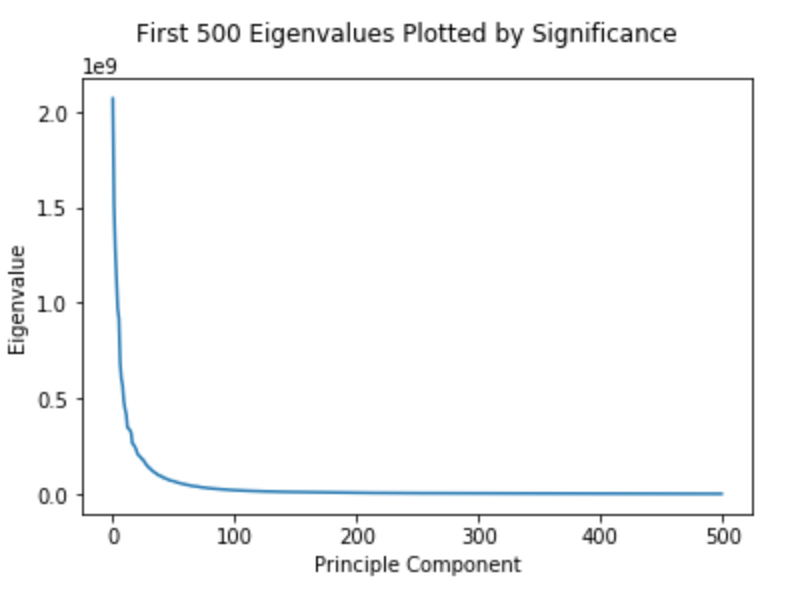
\includegraphics[scale=0.5]{eigenvalues.png} & 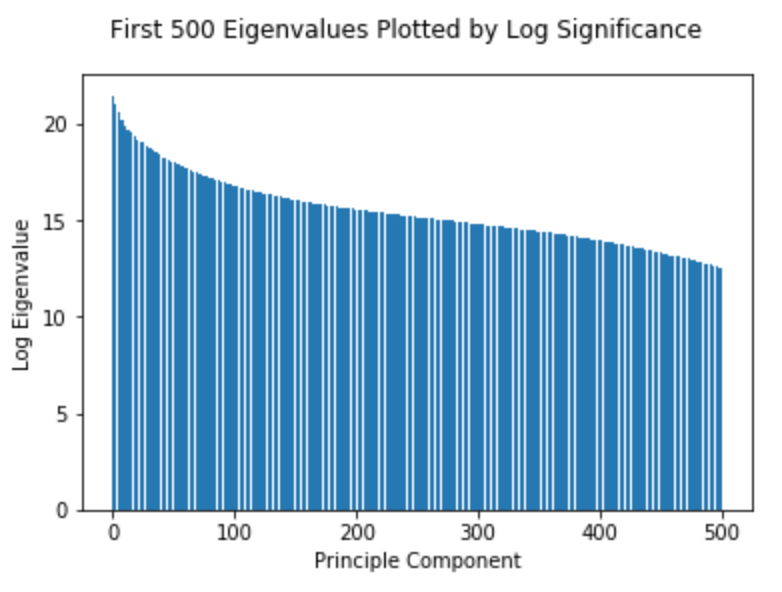
\includegraphics[scale=0.5]{log_eigenvalues.png} \\
  Eigenvalues for the first 500 PC's  & Log Eigenvalues for the first 500 PC's \\
\end{tabular}

\end{center}

Furthermore, graphing the cumulative proportion of variance explained by the first $k$ most significant components shows how this proportion grows rapidly and approaches 1 asymptotically.

\begin{center}
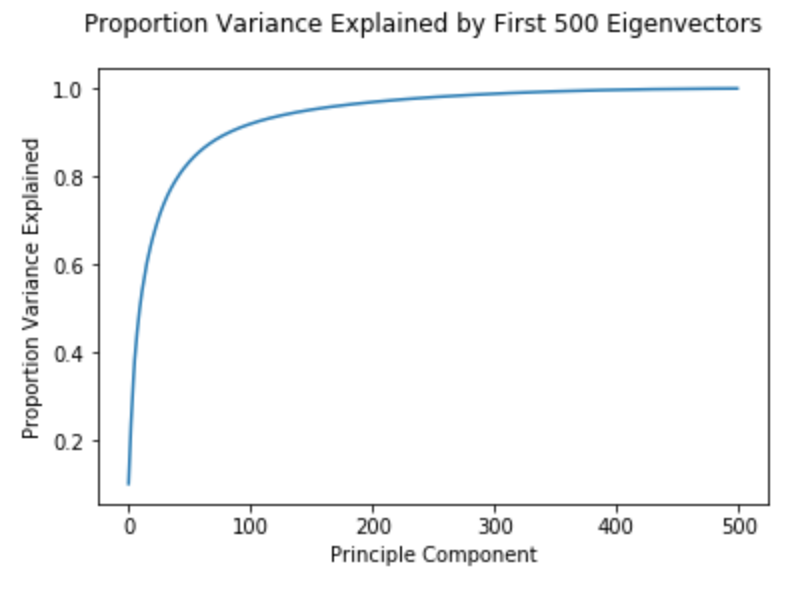
\includegraphics[scale=0.65]{variance.png}
\end{center}

As can be seen, the proportion of variance explained grows rapidly over the first $100$ principle components or so, and reaches a value of about $0.9$ by this point. Then, the proportion grows slower and asymptotically approaches 1. By 300 PC's, the proportion of variance explained appears to be nearly 1. Indeed, by the 500'th PC, I found that the proportion of variance explained is $\boxed{0.9994}$, accounting for total variance of $\boxed{20603735864.27}$.

In general, we can conclude that the proportion of variance explained grows with k approaching 1, and in this case it grows very fast at the beginning and then experiences slower asymptotic growth.

\item The mean of the images and the first $10$ most significant components are shown below:

\begin{center}
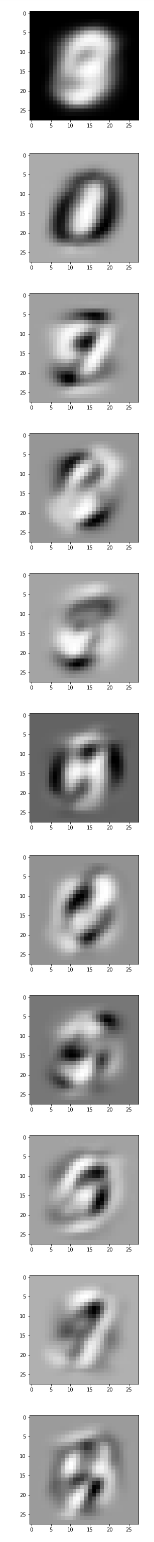
\includegraphics[scale=0.7]{pcs.png}
\end{center}

Unlike the cluster centers for Kmeans, the principle components appear less similar to handwritten digits for the majority of the images. Some of the images still resemble digits, such as 0 and 9 (somewhat). Overall, I would describe these components as resembling digits (or their negated images) or mixtures of digits (or negated mixtures of digits). It makes sense that some of the PC's seem to be negated because the PC's would still be valid if we multiplied by an overall constant of $-1$. (They would still be orthonormal). It seems feasible that these images could be overlayed (e.g. a linear combination) to approximate different digits in the data set! And of course, the mean of the data simply resembles a very blurry mixture of all 10 digits. 

\item The reconstruction error of the data set using the mean image as the approximation of each data point is $\boxed{11024181.94 \approx 1.1 \times 10^{7}}$ and the reconstruction error using the first 10 principle components is $\boxed{7777920.42 \approx 7.8 \times 10^6}$. For comparison, in the previous theory homework, the Kmeans reconstruction error for $K=10$ was around $0.94\times 10^7$ after convergence. So, we see that simply approximating the data with a single mean performs worse (in agreement with what we found last week since reconstruction error decreases with k) than approximating the date with $K=10$ means. However, reconstructing the data with $10$ principle components performs considerably better than using $K=10$ means, but they are on the same order of magnitude. 

We can gain a little intuition behind why this is the case, although the following is not rigorous. Reconstructing the data with Kmeans only requires 10 $28\times 28$ data points and $6000$ category assignments where as reconstructing the data with 10 PCs requires 10 $28\times 28$ data points (the PCs) and a matrix of size $6000 \times 10$ (the projection of the data onto these PCs). So, we have compressed the data less when we are using 10 PCs and hence it makes intuitive sense that our approximation of the original data is more accurate with this method.

Or, consider that with Kmeans, we only have 10 distinct approximations as to what each data point could be, whereas in PCA we create $6000$ distinct approximations (one for each data point). This is another intuitive way to shed light on why PCA may be doing better (although PCA would still do this with only one PC and presumably we would not out perform the Kmeans approximation in this case).


\end{itemize}


\newpage

\begin{itemize}
    \item Name: Zachary Dietz
    \item Email: zachdietz1@gmail.com
    \item Collaborators: Theo Walker, Kaishu Mason
    \item Approximately how long did this homework take you to complete (in hours): 12
\end{itemize}


\end{document}
